\documentclass{article}
\usepackage{amsmath, amssymb, graphicx, booktabs, array}
\begin{document}
\begin{center}
    
\includegraphics[width=1.2in]{/home/runner/workspace/assets/logo.png} \\[0.4cm]
    {\LARGE \textbf{Year 11 Maths Advanced}} \\[0.2cm]
    {\Large \textbf{Functions & Graphs, Trigonometry Set 1}}
\end{center}
\vspace{0.5cm}
\noindent
\begin{tabular}{@{} p{0.6\textwidth} p{0.4\textwidth} @{}}
\textbf{Student Name:} \rule{5cm}{0.4pt} & \textbf{Class:} \rule{3cm}{0.4pt} \\[0.5cm]
\textbf{Time Allowed:} 201 minutes & \textbf{Total Marks:} 134
\end{tabular}
\vspace{0.5cm}\hrule\vspace{0.5cm}

\section*{Section 1}
\begin{enumerate}
    \item Find the domain and range of the function $f(x) = \sqrt{4 - x^2}$. \hfill \textbf{(2 marks)}
    \vspace{0.5cm}

    \item Solve the equation $|2x - 3| = 7$. \hfill \textbf{(2 marks)}
    \vspace{0.5cm}

    \item Given $f(x) = x^2 - 3x$, evaluate $f(-2)$. \hfill \textbf{(1 mark)}
    \vspace{0.5cm}

    \item State the domain and range of the function $y = \frac{1}{x-3} + 2$. \hfill \textbf{(2 marks)}
    \vspace{0.5cm}

    \item Solve the inequality $3 - 2x < 7$. \hfill \textbf{(1 mark)}
    \vspace{0.5cm}

    \item Let $f(x) = x^2$ and $g(x) = x + 3$. Find the expression for the composite function $f(g(x))$. \hfill \textbf{(1 mark)}
    \vspace{0.5cm}

    \item Show whether the function $f(x) = x^3 - 3x$ is even, odd, or neither. \hfill \textbf{(2 marks)}
    \vspace{0.5cm}

    \item Solve the inequality $|x + 4| \le 3$. Write your answer in interval notation. \hfill \textbf{(2 marks)}
    \vspace{0.5cm}

    \item Sketch the graph of $y = |x - 2|$, labelling the vertex and all intercepts. \hfill \textbf{(2 marks)}
    \vspace{0.5cm}

    \item Find the domain of the function $f(x) = \frac{1}{\sqrt{x^2 - 9}}$. \hfill \textbf{(2 marks)}
    \vspace{0.5cm}

    \item Solve the inequality $|2x - 1| > 5$ and sketch the solution on a real number line. \hfill \textbf{(2 marks)}
    \vspace{0.5cm}

    \item If $f(x) = x^2 + 1$ and $g(x) = \sqrt{x - 1}$, find the domain of the composite function $g(f(x))$. \hfill \textbf{(2 marks)}
    \vspace{0.5cm}

    \item Sketch the parabola $y = (x-1)^2 - 4$, clearly labelling the vertex, axis of symmetry, and all intercepts. \hfill \textbf{(2 marks)}
    \vspace{0.5cm}

    \item Solve the algebraic inequality $\frac{x+2}{x-3} \le 0$. \hfill \textbf{(2 marks)}
    \vspace{0.5cm}

    \item A function is defined by $f(x) = \frac{x}{x-1}$ for $x \neq 1$. Show that $f(f(x)) = x$. \hfill \textbf{(2 marks)}
    \vspace{0.5cm}

    \item Determine the range of the function $y = 3 - |x + 1|$. \hfill \textbf{(2 marks)}
    \vspace{0.5cm}

    \item Sketch the graph of the piecewise function:
    \begin{equation*}
    f(x) = \begin{cases} -x - 1, & \text{if } x < 0 \\ x^2 - 1, & \text{if } x \ge 0 \end{cases}
    \end{equation*} \hfill \textbf{(2 marks)}
    \vspace{0.5cm}

    \item The graph of $y = f(x)$ is reflected in the $y$-axis and then translated 3 units vertically upwards. Write down the equation of the resulting graph in terms of $f(x)$. \hfill \textbf{(2 marks)}
    \vspace{0.5cm}

    \item Solve the equation $x^2 - 4 = |x + 2|$. \hfill \textbf{(2 marks)}
    \vspace{0.5cm}

    \item Find the domain and range of the function $y = -\sqrt{2x + 6}$. \hfill \textbf{(2 marks)}
    \vspace{0.5cm}

    \item Solve the inequality $x^2 - 5x + 6 > |x - 3|$. \hfill \textbf{(3 marks)}
    \vspace{0.5cm}

    \item Let $f(x) = \frac{1}{x}$ and $g(x) = 1 - x^2$. Determine the domain and range of the composite function $(f \circ g)(x)$. \hfill \textbf{(3 marks)}
    \vspace{0.5cm}

    \item Sketch the region in the Cartesian plane defined by the inequalities $y \ge x^2 - 4$ and $y \le |x|$ simultaneously. \hfill \textbf{(3 marks)}
    \vspace{0.5cm}

    \item Find all values of the constant $k$ for which the quadratic equation $x^2 - (k-2)x + 9 = 0$ has no real roots. \hfill \textbf{(3 marks)}
    \vspace{0.5cm}

    \item Find the rule, domain, and range for the inverse function $f^{-1}(x)$, given $f(x) = \frac{2x+1}{x-3}$. \hfill \textbf{(3 marks)}
    \vspace{0.5cm}

    \item Solve the inequality $\frac{|x - 2|}{x^2 - 4} \ge 1$. \hfill \textbf{(3 marks)}
    \vspace{0.5cm}

    \item Consider the functions $f(x) = \sqrt{x}$ and $g(x) = x^2 - 4x + 3$. Find the exact domain of the composite function $(f \circ g)(x)$. \hfill \textbf{(3 marks)}
    \vspace{0.5cm}

    \item A function $f(x)$ satisfies the functional equation $f(x) + 2f(1-x) = x^2$ for all real $x$. Determine the explicit algebraic expression for $f(x)$. \hfill \textbf{(3 marks)}
    \vspace{0.5cm}

    \item Find all values of the gradient $m$ for which the line $y = mx - 5$ does not intersect the parabola $y = x^2 - 2x - 1$. \hfill \textbf{(3 marks)}
    \vspace{0.5cm}

    \item Sketch the graph of $y = \frac{|x^2 - 1|}{x - 1}$. Clearly label any intercepts, asymptotes, or holes (points of discontinuity). \hfill \textbf{(3 marks)}
    \vspace{0.5cm}
\end{enumerate}

\section*{Section 2}
\begin{enumerate}
    
    \item Convert the angle $225^\circ$ to radians, expressing your answer in terms of $\pi$. \hfill \textbf{(1 mark)}
    \vspace{0.5cm}

    \item Find the exact value of $\sin\left(\frac{5\pi}{3}\right)$. \hfill \textbf{(1 mark)}
    \vspace{0.5cm}

    \item Solve the trigonometric equation $\cos \theta = -\frac{1}{2}$ for $0 \le \theta \le 2\pi$. \hfill \textbf{(2 marks)}
    \vspace{0.5cm}

    \item Find the length of the unknown side $x$ in the triangle shown below:
    
    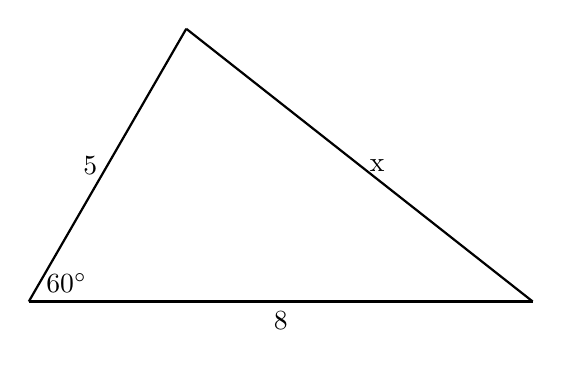
\begin{tikzpicture}[scale=0.8]
    \coordinate (A) at (0,0);
    \coordinate (B) at (8,0);
    \coordinate (C) at (2.5, 4.33);
    \draw[thick] (A) -- (B) node[midway, below] {8};
    \draw[thick] (B) -- (C) node[midway, right] {x};
    \draw[thick] (C) -- (A) node[midway, left] {5};
    \node at (0.6, 0.3) {$60^\circ$};
    \end{tikzpicture} \hfill \textbf{(2 marks)}
    \vspace{0.5cm}

    \item State the amplitude and period of the function $y = 3\sin(2x)$. \hfill \textbf{(2 marks)}
    \vspace{0.5cm}

    \item Simplify the trigonometric expression $\frac{\sin(\pi - \theta)}{\sin(\frac{\pi}{2} - \theta)}$. \hfill \textbf{(2 marks)}
    \vspace{0.5cm}

    \item In $\triangle ABC$, side $a = 7\text{ cm}$, side $b = 10\text{ cm}$, and $\angle C = 45^\circ$. Find the exact area of the triangle. \hfill \textbf{(2 marks)}
    \vspace{0.5cm}

    \item Given that $\tan \theta = -\frac{3}{4}$ and $\frac{\pi}{2} < \theta < \pi$, find the exact value of $\cos \theta$. \hfill \textbf{(2 marks)}
    \vspace{0.5cm}

    \item Solve $2\sin \theta - 1 = 0$ for $0^\circ \le \theta \le 360^\circ$. \hfill \textbf{(2 marks)}
    \vspace{0.5cm}

    \item Use complementary angle results to simplify the expression $\cos(90^\circ - \theta)\tan(\theta)$. \hfill \textbf{(1 mark)}
    \vspace{0.5cm}

    \item Solve the equation $\tan^2 \theta - 3 = 0$ for $0 \le \theta \le 2\pi$. \hfill \textbf{(2 marks)}
    \vspace{0.5cm}

    \item Prove the identity $\frac{1}{1 - \sin \theta} + \frac{1}{1 + \sin \theta} = 2\sec^2 \theta$. \hfill \textbf{(2 marks)}
    \vspace{0.5cm}

    \item Find the exact value of $\cos\left(-\frac{7\pi}{6}\right)$. \hfill \textbf{(2 marks)}
    \vspace{0.5cm}

    \item In $\triangle ABC$, $a = 8\text{ cm}$, $b = 12\text{ cm}$, and $\angle A = 30^\circ$. Find all possible values of $\angle B$ to the nearest degree. \hfill \textbf{(2 marks)}
    \vspace{0.5cm}

    \item Solve the equation $2\cos^2 \theta + \sin \theta - 1 = 0$ for $0^\circ \le \theta \le 360^\circ$. \hfill \textbf{(2 marks)}
    \vspace{0.5cm}

    \item Sketch the graph of $y = 2\cos(x) + 1$ for $0 \le x \le 2\pi$. \hfill \textbf{(2 marks)}
    \vspace{0.5cm}

    \item A sector of a circle of radius $6\text{ cm}$ has an arc length of $4\pi\text{ cm}$. Find the exact area of the sector in terms of $\pi$. \hfill \textbf{(2 marks)}
    \vspace{0.5cm}

    \item Solve the equation $\sin\left(2\theta - \frac{\pi}{4}\right) = \frac{\sqrt{3}}{2}$ for $0 \le \theta \le \pi$. \hfill \textbf{(2 marks)}
    \vspace{0.5cm}

    \item Express the trigonometric expression $\cos\theta + \sin\theta\tan\theta$ as a single trigonometric ratio. \hfill \textbf{(2 marks)}
    \vspace{0.5cm}

    \item An observer standing on top of a vertical cliff of height $50\text{ m}$ looks down at a boat on the sea. The angle of depression is $20^\circ$. Find the horizontal distance of the boat from the base of the cliff, rounded to $1$ decimal place.
    
    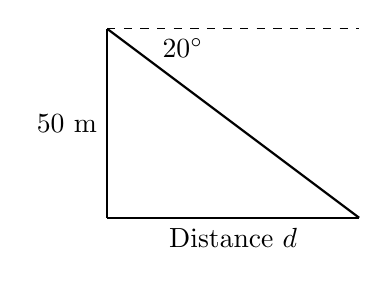
\begin{tikzpicture}[scale=0.8]
    \draw[thick] (0,0) -- (4,0) node[midway, below] {Distance $d$};
    \draw[thick] (0,0) -- (0,3) node[midway, left] {50 m};
    \draw[dashed] (0,3) -- (4,3);
    \draw[thick] (0,3) -- (4,0);
    \node at (1.2, 2.7) {$20^\circ$};
    \end{tikzpicture} \hfill \textbf{(2 marks)}
    \vspace{0.5cm}

    \item Solve the equation $2\sin^2 \theta - 5\sin \theta \cos \theta + 2\cos^2 \theta = 0$ for $0 \le \theta \le \pi$. \hfill \textbf{(3 marks)}
    \vspace{0.5cm}

    \item Prove the trigonometric identity: $\frac{\sin \theta}{1 + \cos \theta} + \frac{1 + \cos \theta}{\sin \theta} = 2\csc \theta$. \hfill \textbf{(3 marks)}
    \vspace{0.5cm}

    \item Sketch the graph of $y = 3\sin\left(2x - \frac{\pi}{2}\right)$ for $0 \le x \le \pi$, labelling all intercepts, the amplitude, and the phase shift. \hfill \textbf{(3 marks)}
    \vspace{0.5cm}

    \item In $\triangle ABC$, the side lengths are $a = x+1$, $b = x$, and $c = x-1$. If the largest angle of this triangle is $120^\circ$, find the value of $x$. \hfill \textbf{(3 marks)}
    \vspace{0.5cm}

    \item Solve the equation $\sqrt{3}\sin\theta - \cos\theta = 0$ for $0 \le \theta \le 2\pi$. \hfill \textbf{(3 marks)}
    \vspace{0.5cm}

    \item Prove that for any triangle $ABC$, the following identity holds:
    \begin{equation*}
    a^2 + b^2 + c^2 = 2(bc\cos A + ac\cos B + ab\cos C)
    \end{equation*} \hfill \textbf{(3 marks)}
    \vspace{0.5cm}

    \item Determine the number of solutions to the equation $\sin x = \frac{x}{10}$ for $x \in \mathbb{R}$. \hfill \textbf{(3 marks)}
    \vspace{0.5cm}

    \item In a triangle $ABC$, the sine values of the angles satisfy the ratio $\sin A : \sin B : \sin C = 4 : 5 : 6$. Find the exact value of $\cos A$. \hfill \textbf{(3 marks)}
    \vspace{0.5cm}

    \item Show that the equation $\cos\theta - \sin\theta = \sqrt{2}$ has only one solution in the interval $0 \le \theta \le 2\pi$, and find this solution. \hfill \textbf{(3 marks)}
    \vspace{0.5cm}

    \item In $\triangle ABC$, the side lengths $a, b, c$ form an arithmetic progression with common difference $d > 0$. If the maximum angle of the triangle is $120^\circ$, prove that the side lengths must be in the ratio $3 : 5 : 7$. \hfill \textbf{(3 marks)}
    \vspace{0.5cm}
\end{enumerate}
\newpage
\begin{center}\Large \textbf{ANSWERS}\end{center}\vspace{0.2cm}\hrule\vspace{0.5cm}
\section*{Section 1}
\begin{enumerate}
    \item Domain: $[-2, 2]$, Range: $[0, 2]$
    \item $x = -2$ or $x = 5$
    \item $10$
    \item Domain: $\{x: x \neq 3\}$, Range: $\{y: y \neq 2\}$
    \item $x > -2$
    \item $f(g(x)) = (x+3)^2$
    \item Odd
    \item $[-7, -1]$
    \item Vertex: $(2,0)$, $y$-intercept: $(0,2)$
    \item $x < -3$ or $x > 3$
    \item $x < -2$ or $x > 3$
    \item Domain: $\mathbb{R}$
    \item Vertex: $(1,-4)$, Intercepts: $(-1,0), (3,0), (0,-3)$
    \item $-2 \le x < 3$
    \item $f(f(x)) = x$
    \item Range: $y \le 3$
    \item Piecewise plot with continuous joint at $(0,-1)$
    \item $y = f(-x) + 3$
    \item $x = -2, 3$
    \item Domain: $x \ge -3$, Range: $y \le 0$
    \item $x < 1$ or $x > 3$
    \item Domain: $\{x: x \neq \pm 1\}$, Range: $y < 0$ or $y \ge 1$
    \item Shaded region bounded by $y = x^2-4$ and $y = |x|$
    \item $-4 < k < 8$
    \item $f^{-1}(x) = \frac{3x+1}{x-2}$, Domain: $x \neq 2$, Range: $y \neq 3$
    \item $-3 \le x < -2$
    \item $x \le 1$ or $x \ge 3$
    \item $f(x) = \frac{x^2 - 4x + 2}{3}$
    \item $-6 < m < 2$
    \item Discontinuity/hole at $(1,-2)$ and $(1,2)$, line segments $y=x+1$ and $y=-x-1$
\end{enumerate}

\section*{Section 2}
\begin{enumerate}
    
    \item $\frac{5\pi}{4}$
    \item $-\frac{\sqrt{3}}{2}$
    \item $\theta = \frac{2\pi}{3}, \frac{4\pi}{3}$
    \item $7$
    \item Amplitude: $3$, Period: $\pi$
    \item $\tan \theta$
    \item $\frac{35\sqrt{2}}{2} \text{ cm}^2$
    \item $-\frac{4}{5}$
    \item $\theta = 30^\circ, 150^\circ$
    \item $\sin\theta\tan\theta$
    \item $\theta = \frac{\pi}{3}, \frac{2\pi}{3}, \frac{4\pi}{3}, \frac{5\pi}{3}$
    \item $2\sec^2 \theta$
    \item $-\frac{\sqrt{3}}{2}$
    \item $B = 49^\circ$ or $131^\circ$
    \item $\theta = 90^\circ, 210^\circ, 330^\circ$
    \item Cosine wave between $y=-1$ and $y=3$
    \item $12\pi \text{ cm}^2$
    \item $\theta = \frac{7\pi}{24}, \frac{11\pi}{24}$
    \item $\sec \theta$
    \item $137.4 \text{ m}$
    \item $\theta \approx 0.46 \text{ rad}, 1.11 \text{ rad}$
    \item $2\csc \theta$
    \item Wave with amplitude $3$, period $\pi$, shifted right by $\frac{\pi}{4}$
    \item $x = 2.5$
    \item $\theta = \frac{\pi}{6}, \frac{7\pi}{6}$
    \item Sum of three cosine rules
    \item $7$
    \item $\frac{3}{4}$
    \item $\theta = \frac{7\pi}{4}$
    \item Side ratio $3:5:7$ from arithmetic progression substitution
\end{enumerate}
\newpage
\begin{center}\Large \textbf{FULLY WORKED SOLUTIONS}\end{center}\vspace{0.2cm}\hrule\vspace{0.5cm}
\section*{Section 1}
\begin{enumerate}
    \item For $f(x) = \sqrt{4-x^2}$, domain requires $4-x^2 \ge 0 \implies x^2 \le 4 \implies -2 \le x \le 2$. Since $\sqrt{4-x^2} \ge 0$ and its maximum value occurs at $x=0$ where $f(0)=2$, the range is $[0, 2]$.
    \vspace{0.5cm}

    \item $|2x - 3| = 7 \implies 2x - 3 = 7$ or $2x - 3 = -7$.
    If $2x - 3 = 7 \implies 2x = 10 \implies x = 5$.
    If $2x - 3 = -7 \implies 2x = -4 \implies x = -2$.
    \vspace{0.5cm}

    \item $f(-2) = (-2)^2 - 3(-2) = 4 + 6 = 10$.
    \vspace{0.5cm}

    \item For $y = \frac{1}{x-3} + 2$, the denominator cannot be zero, so $x-3 \neq 0 \implies$ Domain is $x \neq 3$.
    Since $\frac{1}{x-3} \neq 0$, $y$ cannot equal $2 \implies$ Range is $y \neq 2$.
    \vspace{0.5cm}

    \item $3 - 2x < 7 \implies -2x < 4 \implies x > -2$.
    \vspace{0.5cm}

    \item $f(g(x)) = f(x+3) = (x+3)^2 = x^2 + 6x + 9$.
    \vspace{0.5cm}

    \item $f(-x) = (-x)^3 - 3(-x) = -x^3 + 3x = -(x^3 - 3x) = -f(x)$. Since $f(-x) = -f(x)$, the function is odd.
    \vspace{0.5cm}

    \item $|x+4| \le 3 \implies -3 \le x+4 \le 3 \implies -7 \le x \le -1$. In interval notation: $[-7, -1]$.
    \vspace{0.5cm}

    \item 
    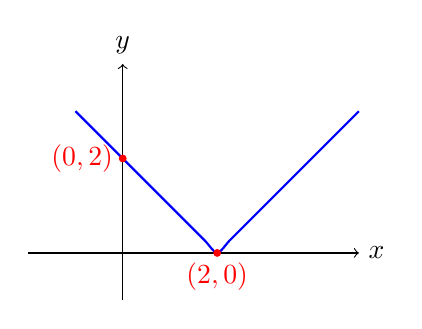
\begin{tikzpicture}[scale=0.6]
    \draw[->] (-2,0) -- (5,0) node[right] {$x$};
    \draw[->] (0,-1) -- (0,4) node[above] {$y$};
    \draw[domain=-1:5, smooth, variable=\x, blue, thick] plot ({\x}, {abs(\x - 2)});
    \filldraw[red] (2,0) circle (2pt) node[below] {$(2,0)$};
    \filldraw[red] (0,2) circle (2pt) node[left] {$(0,2)$};
    \end{tikzpicture}
    \vspace{0.5cm}

    \item For $f(x) = \frac{1}{\sqrt{x^2 - 9}}$, we require $x^2 - 9 > 0 \implies (x-3)(x+3) > 0 \implies x < -3$ or $x > 3$.
    \vspace{0.5cm}

    \item $|2x - 1| > 5 \implies 2x - 1 > 5$ or $2x - 1 < -5$.
    If $2x > 6 \implies x > 3$.
    If $2x < -4 \implies x < -2$.
    \vspace{0.5cm}

    \item $g(f(x)) = g(x^2 + 1) = \sqrt{(x^2+1) - 1} = \sqrt{x^2} = |x|$.
    Since $x^2 \ge 0$, the domain of $g(f(x))$ is all real numbers $\mathbb{R}$.
    \vspace{0.5cm}

    \item $y = (x-1)^2 - 4$. Vertex is at $(1, -4)$.
    $y$-intercept occurs at $x=0 \implies y = -3$.
    $x$-intercepts occur at $y=0 \implies (x-1)^2 = 4 \implies x-1 = \pm 2 \implies x = 3$ or $x = -1$.
    \vspace{0.5cm}

    \item $\frac{x+2}{x-3} \le 0$. The critical points are $x = -2$ (where the numerator is 0) and $x = 3$ (where the denominator is 0). Testing the intervals:
    For $x < -2$, $\frac{-}{-} > 0$.
    For $-2 \le x < 3$, $\frac{+}{-} \le 0$.
    For $x > 3$, $\frac{+}{+} > 0$.
    Thus, $-2 \le x < 3$.
    \vspace{0.5cm}

    \item $f(f(x)) = f\left(\frac{x}{x-1}\right) = \frac{\frac{x}{x-1}}{\frac{x}{x-1} - 1} = \frac{\frac{x}{x-1}}{\frac{x - (x-1)}{x-1}} = \frac{x}{1} = x$.
    \vspace{0.5cm}

    \item Since $|x+1| \ge 0$ for all real $x$, $-|x+1| \le 0 \implies 3 - |x+1| \le 3$. Thus, the range is $y \le 3$.
    \vspace{0.5cm}

    \item 
    \begin{tikzpicture}[scale=0.6]
    \draw[->] (-3,0) -- (3,0) node[right] {$x$};
    \draw[->] (0,-2) -- (0,4) node[above] {$y$};
    \draw[domain=-2:0, smooth, variable=\x, blue, thick] plot ({\x}, {-\x - 1});
    \draw[domain=0:2, smooth, variable=\x, blue, thick] plot ({\x}, {\x*\x - 1});
    \filldraw[blue] (0,-1) circle (2pt);
    \end{tikzpicture}
    \vspace{0.5cm}

    \item Reflection in the $y$-axis changes $f(x)$ to $f(-x)$. A translation 3 units upwards changes this to $y = f(-x) + 3$.
    \vspace{0.5cm}

    \item $x^2 - 4 = |x + 2|$.
    Case 1: $x \ge -2 \implies x^2 - 4 = x + 2 \implies x^2 - x - 6 = 0 \implies (x-3)(x+2) = 0 \implies x = 3$ or $x = -2$ (both valid).
    Case 2: $x < -2 \implies x^2 - 4 = -(x+2) \implies x^2 + x - 2 = 0 \implies (x+2)(x-1) = 0 \implies x = -2$ or $x = 1$ (neither is $< -2$).
    Solutions: $x = -2, 3$.
    \vspace{0.5cm}

    \item For $y = -\sqrt{2x+6}$, we need $2x+6 \ge 0 \implies x \ge -3$. The range is $y \le 0$ because of the negative sign before the square root.
    \vspace{0.5cm}

    \item $x^2 - 5x + 6 > |x - 3| \implies (x-2)(x-3) > |x-3|$.
    If $x \ge 3 \implies (x-2)(x-3) > x-3 \implies (x-3)(x-3) > 0 \implies (x-3)^2 > 0 \implies x > 3$.
    If $x < 3 \implies (x-2)(x-3) > -(x-3) \implies (x-3)(x-1) > 0$. Since $x-3 < 0$, we must have $x-1 < 0 \implies x < 1$.
    Thus, $x < 1$ or $x > 3$.
    \vspace{0.5cm}

    \item $(f \circ g)(x) = \frac{1}{1 - x^2}$.
    Domain: $1 - x^2 \neq 0 \implies x \neq \pm 1$.
    Range: Let $y = \frac{1}{1-x^2}$. Since $x^2 \ge 0$ ($x \neq \pm 1$), $1-x^2 < 1$.
    If $0 < 1-x^2 < 1 \implies y > 1$.
    If $1-x^2 < 0 \implies y < 0$.
    At $x=0$, $y=1$. Thus, the range is $y < 0$ or $y \ge 1$.
    \vspace{0.5cm}

    \item 
    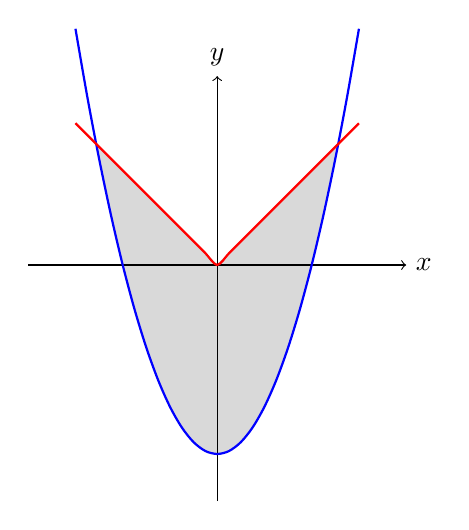
\begin{tikzpicture}[scale=0.6]
    \filldraw[gray!30, domain=-2.56:2.56] plot (\x, {\x*\x - 4}) -- plot[domain=2.56:-2.56] (\x, {abs(\x)});
    \draw[->] (-4,0) -- (4,0) node[right] {$x$};
    \draw[->] (0,-5) -- (0,4) node[above] {$y$};
    \draw[domain=-3:3, smooth, variable=\x, blue, thick] plot ({\x}, {\x*\x - 4});
    \draw[domain=-3:3, smooth, variable=\x, red, thick] plot ({\x}, {abs(\x)});
    \end{tikzpicture}
    \vspace{0.5cm}

    \item No real roots $\implies \Delta < 0 \implies (k-2)^2 - 4(1)(9) < 0 \implies (k-2)^2 < 36 \implies -6 < k-2 < 6 \implies -4 < k < 8$.
    \vspace{0.5cm}

    \item Swap $x$ and $y$: $x = \frac{2y+1}{y-3} \implies x(y-3) = 2y + 1 \implies y(x-2) = 3x+1 \implies y = \frac{3x+1}{x-2}$.
    Rule: $f^{-1}(x) = \frac{3x+1}{x-2}$.
    Domain of $f^{-1}$ is the range of $f \implies x \neq 2$.
    Range of $f^{-1}$ is the domain of $f \implies y \neq 3$.
    \vspace{0.5cm}

    \item $\frac{|x - 2|}{(x-2)(x+2)} \ge 1$. Note $x \neq \pm 2$.
    If $x > 2 \implies \frac{x-2}{(x-2)(x+2)} = \frac{1}{x+2} \ge 1 \implies x+2 \le 1 \implies x \le -1$ (no solution since $x > 2$).
    If $x < 2$ (and $x \neq -2$) $\implies \frac{-(x-2)}{(x-2)(x+2)} = \frac{-1}{x+2} \ge 1$. Since LHS must be positive, $x+2 < 0 \implies x < -2$. Thus $-1 \le x+2 \implies x \ge -3$.
    So, $-3 \le x < -2$.
    \vspace{0.5cm}

    \item $(f \circ g)(x) = \sqrt{x^2 - 4x + 3}$.
    Domain requires $x^2 - 4x + 3 \ge 0 \implies (x-1)(x-3) \ge 0 \implies x \le 1$ or $x \ge 3$.
    \vspace{0.5cm}

    \item Given (1) $f(x) + 2f(1-x) = x^2$.
    Substitute $x \leftarrow 1-x$: (2) $f(1-x) + 2f(x) = (1-x)^2 = x^2 - 2x + 1$.
    Multiply (2) by 2: $2f(1-x) + 4f(x) = 2x^2 - 4x + 2$.
    Subtract (1) from this: $3f(x) = x^2 - 4x + 2 \implies f(x) = \frac{x^2 - 4x + 2}{3}$.
    \vspace{0.5cm}

    \item $x^2 - 2x - 1 = mx - 5 \implies x^2 - (2+m)x + 4 = 0$.
    No intersection $\implies \Delta < 0 \implies (2+m)^2 - 16 < 0 \implies (2+m)^2 < 16 \implies -4 < 2+m < 4 \implies -6 < m < 2$.
    \vspace{0.5cm}

    \item $y = \frac{|x^2 - 1|}{x - 1}$. Note $x \neq 1$.
    If $x > 1$ or $x \le -1$, $y = \frac{x^2 - 1}{x - 1} = x + 1$.
    If $-1 < x < 1$, $y = \frac{-(x^2 - 1)}{x - 1} = -(x+1) = -x - 1$.
    There are holes at $(1, 2)$ and $(1, -2)$. Intercepts at $(0, -1)$ and $(-1, 0)$.
    \vspace{0.5cm}
\end{enumerate}

\section*{Section 2}
\begin{enumerate}
    
    \item $225^\circ \times \frac{\pi}{180^\circ} = \frac{5\pi}{4}$ radians.
    \vspace{0.5cm}

    \item $\sin\left(\frac{5\pi}{3}\right) = -\sin\left(\frac{\pi}{3}\right) = -\frac{\sqrt{3}}{2}$ (since $\frac{5\pi}{3}$ is in the 4th quadrant).
    \vspace{0.5cm}

    \item $\cos\theta = -\frac{1}{2}$. The reference angle is $\frac{\pi}{3}$. In quadrants 2 and 3:
    $\theta = \pi - \frac{\pi}{3} = \frac{2\pi}{3}$ and $\theta = \pi + \frac{\pi}{3} = \frac{4\pi}{3}$.
    \vspace{0.5cm}

    \item By the Cosine Rule:
    $x^2 = 5^2 + 8^2 - 2(5)(8)\cos(60^\circ) = 25 + 64 - 80(0.5) = 89 - 40 = 49 \implies x = 7$.
    \vspace{0.5cm}

    \item For $y = 3\sin(2x)$, Amplitude $= 3$. Period $= \frac{2\pi}{2} = \pi$.
    \vspace{0.5cm}

    \item $\frac{\sin(\pi - \theta)}{\sin(\frac{\pi}{2} - \theta)} = \frac{\sin \theta}{\cos \theta} = \tan \theta$.
    \vspace{0.5cm}

    \item $\text{Area} = \frac{1}{2}ab\sin C = \frac{1}{2}(7)(10)\sin(45^\circ) = 35 \times \frac{\sqrt{2}}{2} = \frac{35\sqrt{2}}{2} \text{ cm}^2$.
    \vspace{0.5cm}

    \item Since $\frac{\pi}{2} < \theta < \pi$, $\theta$ is in the 2nd quadrant where cosine is negative.
    Using $\tan \theta = -\frac{3}{4}$, the hypotenuse is $5$. Hence, $\cos \theta = -\frac{4}{5}$.
    \vspace{0.5cm}

    \item $2\sin\theta = 1 \implies \sin\theta = \frac{1}{2} \implies \theta = 30^\circ, 150^\circ$.
    \vspace{0.5cm}

    \item $\cos(90^\circ - \theta)\tan(\theta) = \sin\theta\left(\frac{\sin\theta}{\cos\theta}\right) = \sin\theta\tan\theta$.
    \vspace{0.5cm}

    \item $\tan^2 \theta = 3 \implies \tan \theta = \pm \sqrt{3}$. Reference angle is $\frac{\pi}{3}$.
    In all four quadrants: $\theta = \frac{\pi}{3}, \frac{2\pi}{3}, \frac{4\pi}{3}, \frac{5\pi}{3}$.
    \vspace{0.5cm}

    \item LHS $= \frac{(1+\sin\theta) + (1-\sin\theta)}{(1-\sin\theta)(1+\sin\theta)} = \frac{2}{1-\sin^2\theta} = \frac{2}{\cos^2\theta} = 2\sec^2\theta =$ RHS.
    \vspace{0.5cm}

    \item $\cos\left(-\frac{7\pi}{6}\right) = \cos\left(\frac{5\pi}{6}\right) = -\cos\left(\frac{\pi}{6}\right) = -\frac{\sqrt{3}}{2}$.
    \vspace{0.5cm}

    \item By the Sine Rule: $\frac{\sin B}{12} = \frac{\sin 30^\circ}{8} \implies \sin B = \frac{12 \times 0.5}{8} = 0.75$.
    $B_1 \approx 49^\circ$ or $B_2 = 180^\circ - 49^\circ = 131^\circ$. Both are valid since $A + B < 180^\circ$.
    \vspace{0.5cm}

    \item Substitute $\cos^2\theta = 1-\sin^2\theta \implies 2(1-\sin^2\theta) + \sin\theta - 1 = 0 \implies 2\sin^2\theta - \sin\theta - 1 = 0 \implies (2\sin\theta+1)(\sin\theta-1) = 0$.
    If $\sin\theta = 1 \implies \theta = 90^\circ$.
    If $\sin\theta = -0.5 \implies \theta = 210^\circ, 330^\circ$.
    \vspace{0.5cm}

    \item 
    \begin{tikzpicture}[scale=0.6]
    \draw[->] (-0.5,0) -- (7,0) node[right] {$x$};
    \draw[->] (0,-2) -- (0,4) node[above] {$y$};
    \draw[domain=0:6.28, smooth, variable=\x, blue, thick] plot ({\x}, {2*cos(\x r) + 1});
    \draw[dashed] (0,1) -- (6.28,1);
    \end{tikzpicture}
    \vspace{0.5cm}

    \item $l = r\theta \implies 4\pi = 6\theta \implies \theta = \frac{2\pi}{3}$ radians.
    $\text{Area} = \frac{1}{2}r^2\theta = \frac{1}{2}(36)\left(\frac{2\pi}{3}\right) = 12\pi \text{ cm}^2$.
    \vspace{0.5cm}

    \item $\sin\left(2\theta - \frac{\pi}{4}\right) = \frac{\sqrt{3}}{2}$. Since $0 \le \theta \le \pi$, we have $-\frac{\pi}{4} \le 2\theta - \frac{\pi}{4} \le \frac{7\pi}{4}$.
    Thus, $2\theta - \frac{\pi}{4} = \frac{\pi}{3} \implies 2\theta = \frac{7\pi}{12} \implies \theta = \frac{7\pi}{24}$.
    Or $2\theta - \frac{\pi}{4} = \frac{2\pi}{3} \implies 2\theta = \frac{11\pi}{12} \implies \theta = \frac{11\pi}{24}$.
    \vspace{0.5cm}

    \item $\cos\theta + \sin\theta\left(\frac{\sin\theta}{\cos\theta}\right) = \frac{\cos^2\theta + \sin^2\theta}{\cos\theta} = \frac{1}{\cos\theta} = \sec\theta$.
    \vspace{0.5cm}

    \item Let $d$ be the horizontal distance. $\tan(20^\circ) = \frac{50}{d} \implies d = \frac{50}{\tan(20^\circ)} \approx 137.4\text{ m}$.
    \vspace{0.5cm}

    \item Divide by $\cos^2 \theta$: $2\tan^2\theta - 5\tan\theta + 2 = 0 \implies (2\tan\theta-1)(\tan\theta-2) = 0$.
    If $\tan\theta = 0.5 \implies \theta \approx 0.46 \text{ rad}$.
    If $\tan\theta = 2 \implies \theta \approx 1.11 \text{ rad}$.
    \vspace{0.5cm}

    \item LHS $= \frac{\sin^2 \theta + (1+\cos\theta)^2}{\sin\theta(1+\cos\theta)} = \frac{\sin^2\theta + 1 + 2\cos\theta + \cos^2\theta}{\sin\theta(1+\cos\theta)} = \frac{2 + 2\cos\theta}{\sin\theta(1+\cos\theta)} = \frac{2(1+\cos\theta)}{\sin\theta(1+\cos\theta)} = 2\csc \theta =$ RHS.
    \vspace{0.5cm}

    \item $y = 3\sin\left(2(x - \frac{\pi}{4})\right)$. Amplitude $= 3$, Period $= \pi$, Phase shift $= \frac{\pi}{4}$ to the right.
    \vspace{0.5cm}

    \item The largest angle is $120^\circ$, opposite the largest side $a = x+1$.
    By the Cosine Rule: $(x+1)^2 = x^2 + (x-1)^2 - 2x(x-1)\cos(120^\circ)$
    $x^2 + 2x + 1 = x^2 + x^2 - 2x + 1 + x(x-1) \implies 2x^2 - 5x = 0 \implies x = 2.5$ (since $x > 1$ for positive sides).
    \vspace{0.5cm}

    \item $\sqrt{3}\sin\theta = \cos\theta \implies \tan\theta = \frac{1}{\sqrt{3}}$.
    In quadrants 1 and 3: $\theta = \frac{\pi}{6}, \frac{7\pi}{6}$.
    \vspace{0.5cm}

    \item By the Cosine Rule:
    $bc\cos A = \frac{b^2+c^2-a^2}{2}$, $ac\cos B = \frac{a^2+c^2-b^2}{2}$, $ab\cos C = \frac{a^2+b^2-c^2}{2}$.
    Summing these yields:
    $bc\cos A + ac\cos B + ab\cos C = \frac{a^2+b^2+c^2}{2} \implies 2(bc\cos A + ac\cos B + ab\cos C) = a^2+b^2+c^2$.
    \vspace{0.5cm}

    \item The solutions correspond to intersections of $y = \sin x$ and $y = \frac{x}{10}$. Since $|\sin x| \le 1$, intersections must occur in $[-10, 10]$.
    There is 1 solution at $x=0$.
    For $x > 0$, the line crosses the wave once in $[0,\pi]$, and twice in $[2\pi, 3\pi]$ (since $3\pi \approx 9.42 < 10$). Total of 3 positive solutions.
    By symmetry, there are 3 negative solutions. Total $= 1 + 3 + 3 = 7$ solutions.
    \vspace{0.5cm}

    \item By the Sine Rule, $a : b : c = \sin A : \sin B : \sin C = 4 : 5 : 6$. Let $a = 4k, b = 5k, c = 6k$.
    $\cos A = \frac{b^2+c^2-a^2}{2bc} = \frac{25k^2+36k^2-16k^2}{2(5k)(6k)} = \frac{45}{60} = \frac{3}{4}$.
    \vspace{0.5cm}

    \item Divide by $\sqrt{2}$: $\frac{1}{\sqrt{2}}\cos\theta - \frac{1}{\sqrt{2}}\sin\theta = 1 \implies \cos\left(\theta + \frac{\pi}{4}\right) = 1$.
    For $0 \le \theta \le 2\pi \implies \frac{\pi}{4} \le \theta + \frac{\pi}{4} \le \frac{9\pi}{4}$.
    The only solution is $\theta + \frac{\pi}{4} = 2\pi \implies \theta = \frac{7\pi}{4}$.
    \vspace{0.5cm}

    \item Let the side lengths be $x-d, x, x+d$.
    The largest angle is $C = 120^\circ$, opposite to $c = x+d$.
    Cosine Rule: $(x+d)^2 = (x-d)^2 + x^2 - 2x(x-d)\cos(120^\circ) \implies x^2 + 2xd + d^2 = x^2 - 2xd + d^2 + x^2 + x(x-d) \implies 2x^2 - 5xd = 0 \implies x = 2.5d$.
    Hence, side lengths are $1.5d, 2.5d, 3.5d \implies$ ratio is $3:5:7$.
    \vspace{0.5cm}
\end{enumerate}
\end{document}